\documentclass[11pt]{article}
\usepackage[letterpaper, left=1in, right=1in, top=1in, bottom=1.25in]{geometry}

\usepackage{lipsum}  
\usepackage{graphicx}
\graphicspath{{./Figures/}}
\usepackage{fancyhdr}
\usepackage{amsmath}
\usepackage{subfig}
\usepackage{charter} %good loooking font
\usepackage{booktabs} %good looking tables
\usepackage{float} %to allow for figures/tables to be placed exactly
\usepackage{amssymb} %math package

\setlength{\parskip}{1em} % space between paragraphs
\setlength{\parindent}{0em} % no paragraph indentation

\pagestyle{fancy}
\fancyhead[L]{EE 101-01} %class
\fancyhead[C]{A Nifty Title Goes Here} %paper title
\fancyhead[R]{NMT IEEE Student Branch} %your name
\fancyfoot[L]{New Mexico Tech} %our school
\fancyfoot[R]{Fall 2019} % the date
\renewcommand{\headrulewidth}{0.4pt}
\renewcommand{\footrulewidth}{0.4pt}


\title{\LARGE \textbf{A Nifty Title Goes Here} 
        \\ Latex Manuscript (Example)}
\author{NMT IEEE Student Branch
        \\ EE 101-01}
\date{\today}


\begin{document}
\maketitle

\begin{abstract}
    \lipsum[1]
\end{abstract}

\newpage

\tableofcontents
\listoffigures
\listoftables

\newpage

\section*{Introduction}
\lipsum[2]
 
\section{Background}
\lipsum[3-4]

\begin{equation}\label{eq_1}
  H(\omega) =
  \begin{cases}
   1 & |\omega| < \omega_0 \\
   0 & \omega_0 < |\omega| < \pi \\
  \end{cases}
  =
    \begin{cases}
   1 & |\omega| < \omega_0 \\
   0 & \omega_0 < |\omega| < \pi \\
  \end{cases}
\end{equation}

\lipsum[5]

\begin{equation}\label{eq:2}
    h[n] = \frac{1}{2\pi} \int_{-\frac{\pi}{4}}^{\frac{\pi}{4}} e^{j\Omega n} d\omega
\end{equation} 



\section{Case Studies}
\lipsum[6]

\begin{figure}[H]
\centering
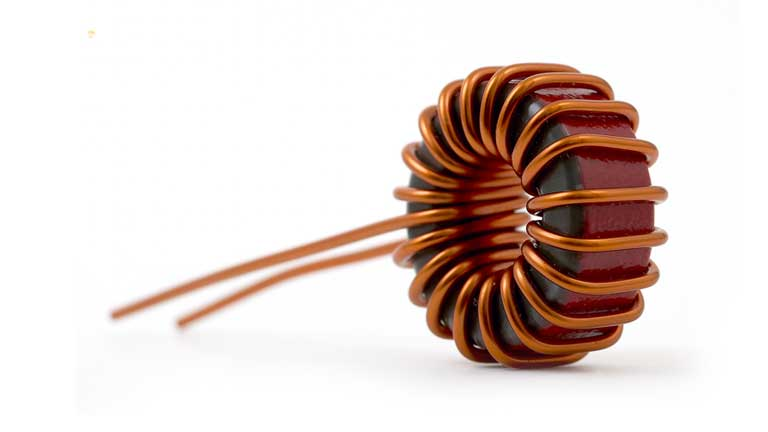
\includegraphics[width=.3\textwidth]{Pictures/ind.jpg}\hfill 
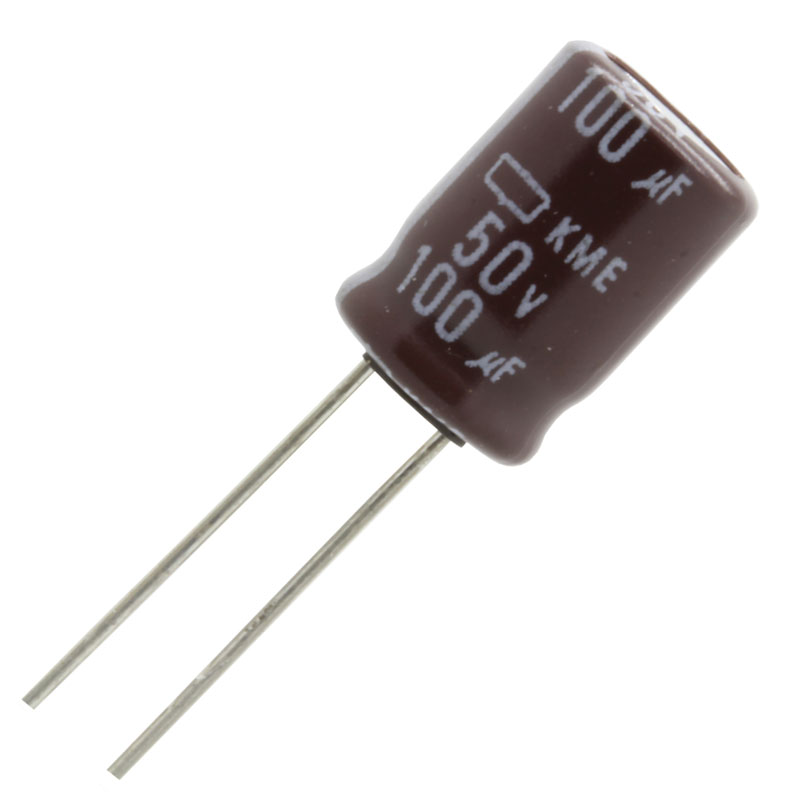
\includegraphics[width=.3\textwidth]{Pictures/cap.jpg}\hfill
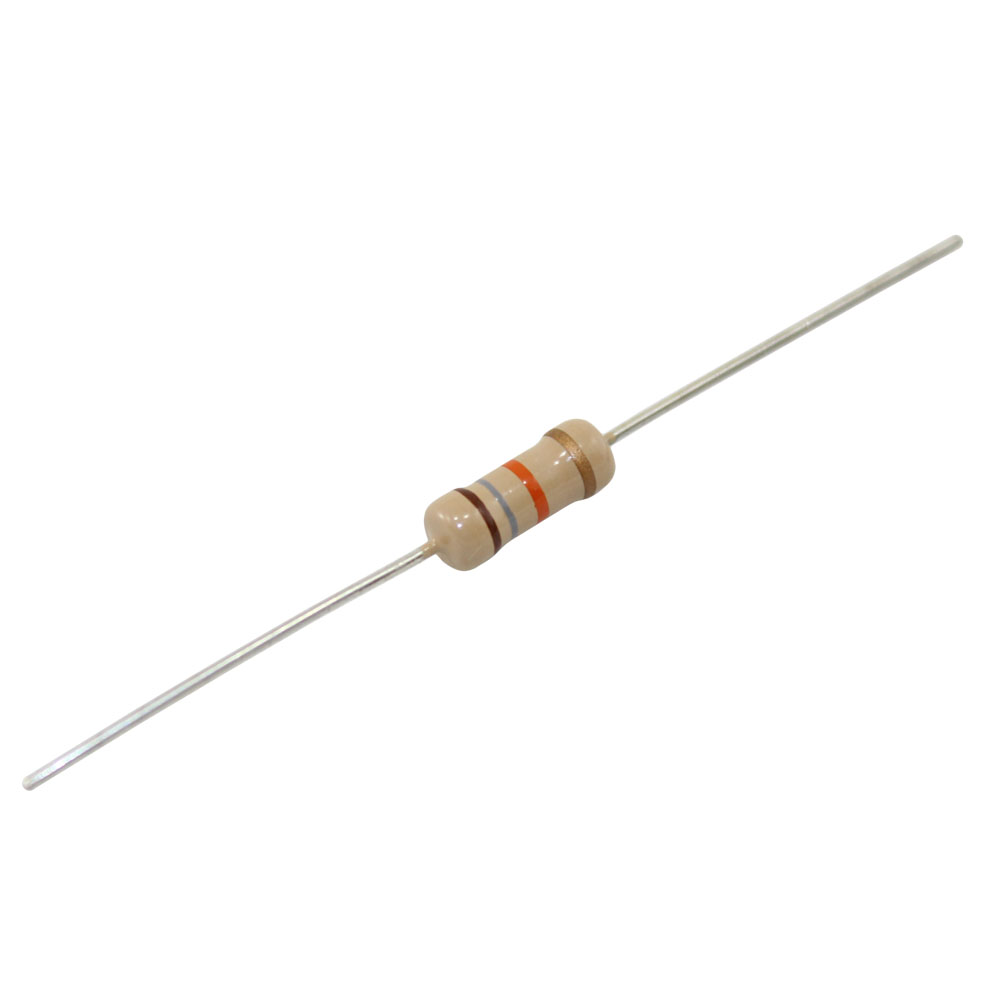
\includegraphics[width=.3\textwidth]{Pictures/res.jpg}
\caption{An inductor, a capacitor, and a resistor}
\label{fig:components}
\end{figure}

\subsection{Windows}
\lipsum[7]

\begin{figure}[H]
	\centering
	
\includegraphics[width=0.5\linewidth]{Pictures/windows.jpg}
	\caption{Windows Logo}
	\label{fig:win}
\end{figure}



\subsection{Linux}
\lipsum[8]

\begin{figure}[H]
	\centering
	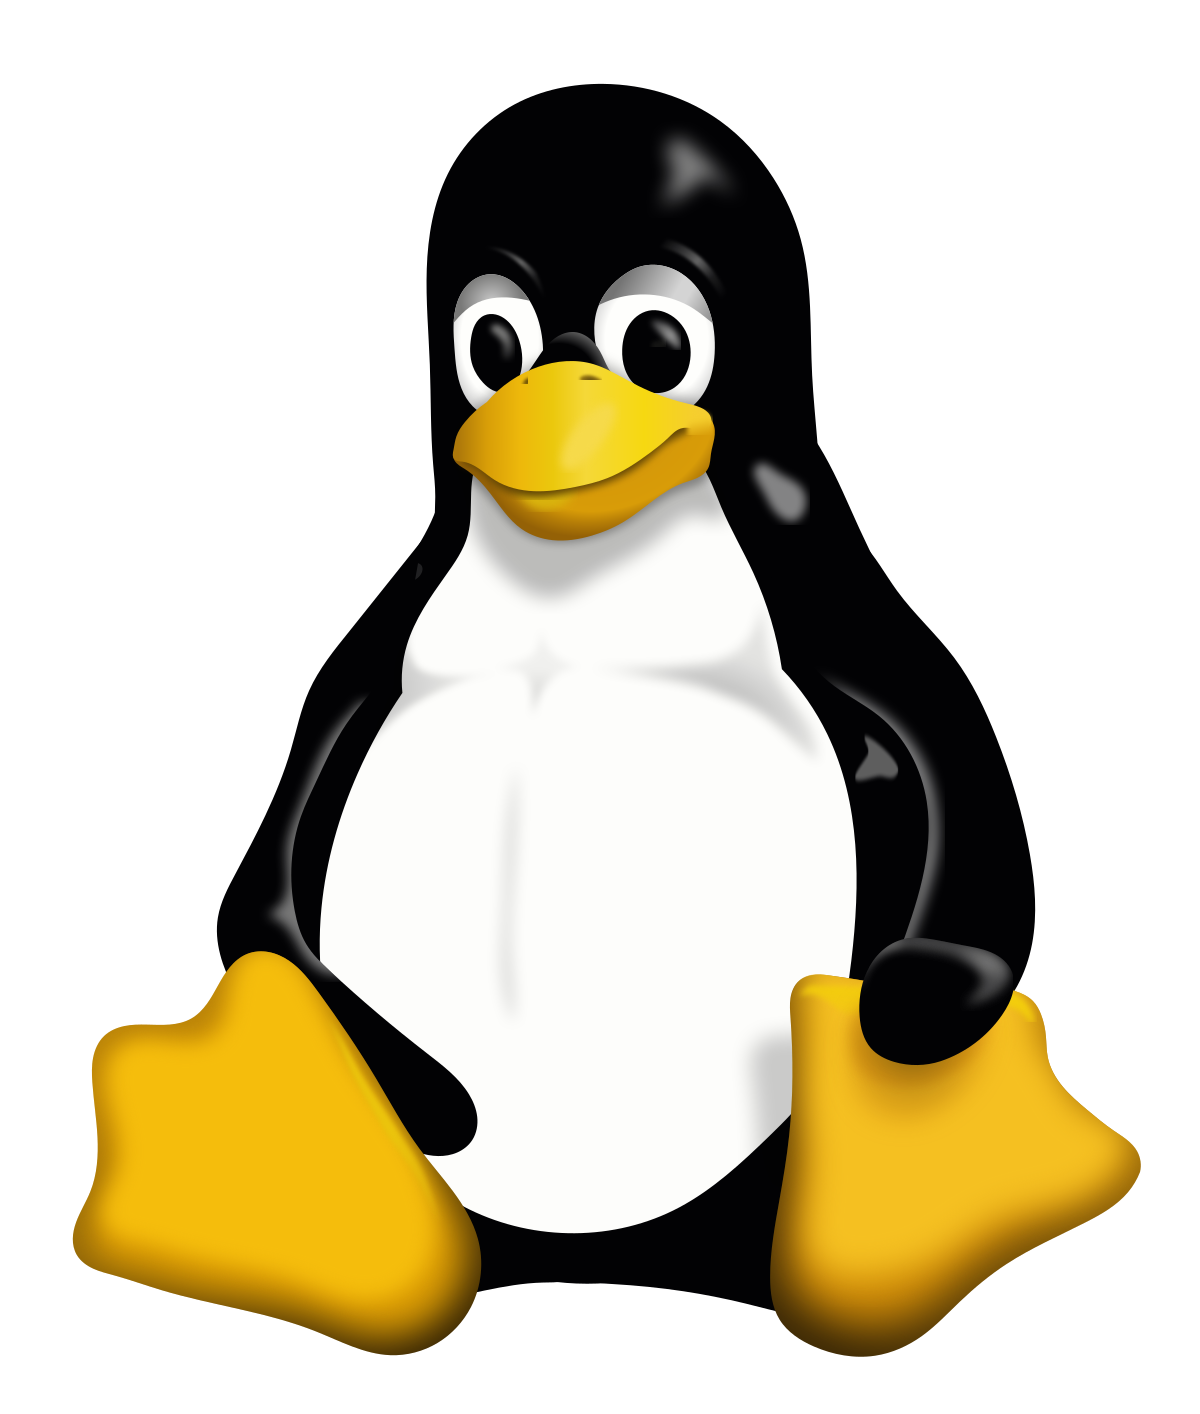
\includegraphics[width=0.25\linewidth]{Pictures/linux.png}
	\caption{Linux Penguin}
	\label{fig:lin}
\end{figure}



\subsection{Mac}
\lipsum[9]

\begin{figure}[H]
	\centering
	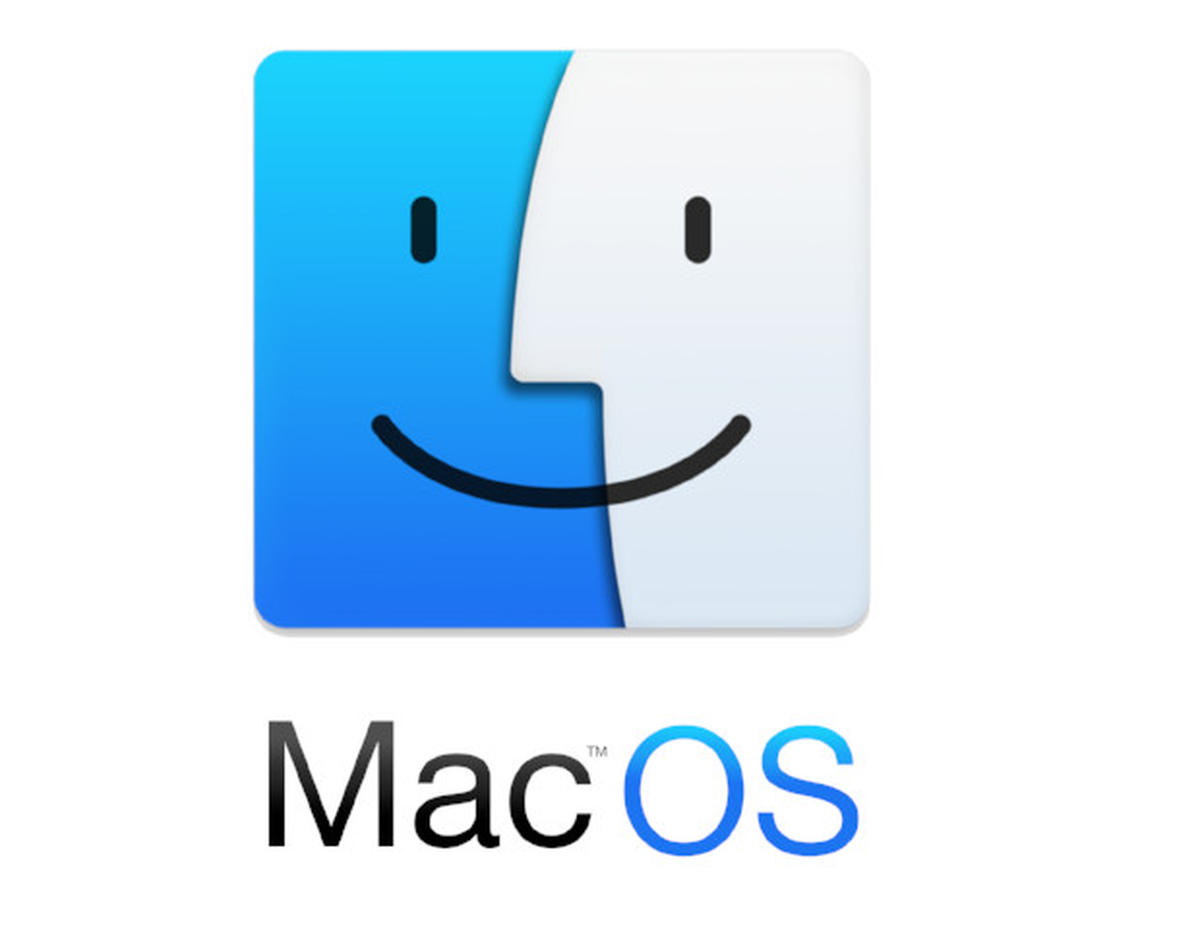
\includegraphics[width=0.25\linewidth]{Pictures/mac.jpg}
	\caption{Mac OS Logo}
	\label{fig:mac}
\end{figure}











\subsection{Results and Analysis}
So this is where there is actually some written content. You can reference Figure \ref{fig:components}, Equation \ref{eq_1}, and Table \ref{tab:1} like this. In text citations can be done like this \cite{b0}. Also, math done outside of and equation \textit{need} \textbf{to} \underline{be} written with \$, like this $\omega 1 _{two}$.




\begin{table}[H]
\centering
\caption{This is a sample table}\label{tab:1}
\begin{tabular}{ |p{3cm}||p{3cm}|p{3cm}|p{3cm}|  }
 \hline
 \multicolumn{4}{|c|}{Country List} \\
 \hline
 Country Name     or Area Name& ISO ALPHA 2 Code &ISO ALPHA 3 Code&ISO numeric Code\\
 \hline
 Afghanistan   & AF    &AFG&   004\\
 Aland Islands&   AX  & ALA   &248\\
 Albania &AL & ALB&  008\\
 Algeria    &DZ & DZA&  012\\
 American Samoa&   AS  & ASM&016\\
 Andorra& AD  & AND   &020\\
 Angola& AO  & AGO&024\\
 \hline
\end{tabular}
\end{table}

\lipsum[4]

\begin{table}[H]
\centering
\caption{This is a different version of the sample table}\label{tab:2}
\begin{tabular}{@{}llll@{}}
 \toprule
 \multicolumn{4}{c}{Country List} \\
 \midrule
 Country Name     or Area Name& ISO ALPHA 2 Code &ISO ALPHA 3 Code&ISO numeric Code\\
 \hline
 Afghanistan   & AF    &AFG&   004\\
 Aland Islands&   AX  & ALA   &248\\
 Albania &AL & ALB&  008\\
 Algeria    &DZ & DZA&  012\\
 American Samoa&   AS  & ASM&016\\
 Andorra& AD  & AND   &020\\
 Angola& AO  & AGO&024\\
 \bottomrule
\end{tabular}
\end{table}

\lipsum[8]



\section{Conclusion}
\lipsum[9]

f;lasjf;lkasjdf



\newpage

\begin{thebibliography}{99}

% https://ieeexplore.ieee.org/document/6518912
\bibitem{b0} A. Rghioui, M. Bouhorma and A. Benslimane, "Analytical study of security aspects in 6LoWPAN networks," 2013 5th International Conference on Information and Communication Technology for the Muslim World (ICT4M), Rabat, 2013, pp. 1-5. Available: ieeexplore.ieee.org. [Accessed: Oct. 17, 2019].

%https://www.cisco.com/c/en/us/products/collateral/ios-nx-os-software/enterprise-ipv6-solution/whitepaper_c11-698132.html
\bibitem{b1} Cisco, "How Can Service Providers Face IPv4 Address Exhaustion," 2012. [Online]. Available: https://www.cisco.com. [Accessed: Oct. 17, 2019].

% https://www.fcc.gov/consumers/guides/internet-protocol-version-6-ipv6-consumers
\bibitem{b2} Federal Communications Commission, "Internet Protocol Version 6: IPv6 for Consumers,"  Consumer and Governmental Affairs, 2017. [Online]. Available: www.fcc.gov. [Accessed: Oct. 17, 2019].


\end{thebibliography}

\newpage

\section*{Appendix}


\end{document}          
